%!TEX program = xelatex
\let\stop\empty

\documentclass[12pt,a4paper]{exam-zh}

\usepackage{xeCJK}
\setCJKmainfont{Noto Serif CJK SC}
\setCJKfamilyfont{zhkai}[AutoFakeBold=2]{FandolKai-Regular}
\usepackage{geometry}
\usepackage{array}
\usepackage{tikz}
\usepackage{amsmath}
\usepackage{wrapfig}
\usepackage{adjustbox}
\usepackage{enumitem}
\usepackage{fancyhdr}

\usepackage{scalerel}
\def\mcirc{\mathbin{\scalerel*{\circ}{j}}}
\def\msquare{\mathord{\scalerel*{\Box}{gX}}}

% \renewcommand{\choiceshook}{%
%     \setlength{\leftmargin}{18pt}%
% }
\geometry{margin=2cm}
\hbadness=10000


% ----------- 调整 exam -----------


% --- 全局样式定义 ---
% 定义选择题环境：题号 1. 2.，选项 A. B. C. D. 粗体，且保留 1.5em 间距
\examsetup{
    page = {
    size = a4paper,           % 设定纸张大小 [4]
    foot-content = { - ; - }  % 页脚显示为 -1-, -2- 格式 [3]
  },
    choices = {
    label-pos = top-left,
    column-sep = 1em,
    label-pos = auto,
    label-sep = 0.5em,
    max-columns = 4
    },
  question = {
    top-sep    = 1em, % 调整题目上方的垂直距离（默认值为 .5em plus .5em minus .2em）
    bottom-sep = 1em  % 调整题目下方的垂直距离（默认值为 .5em plus .5em minus .2em）
  },
    paren = {
    show-paren = false  % 设置为 false 则不显示括号 [3, 4]
  },
    choices = {
    label = \textbf{\Alph*}
  }, 
    solution = {
    show-solution = show-move, % 答案紧跟题目后直接显示
    label-content = {参考答案},  % 答案区的标题文字
    show-qed = true            % 在解答末尾显示结束符号 ◻ 
  }
}



\begin{document}

% ==========================
% 三栏标题区
% ==========================
\noindent
\begin{tabular*}{\textwidth}{@{\extracolsep{\fill}} p{0.28\textwidth} p{0.32\textwidth} p{0.28\textwidth}}

\raggedright
\textbf{高中一}\\[0.2em]
\textbf{}{数学（试卷一）}\\[0.4em]
姓名：\underline{\hspace{3cm}} &

\centering
\textbf{金宝培元独立中学}\\[0.2em]
\textbf{半年考}\\[0.4em]
班级：J1 ( H / I / F ) &

\raggedright
日期：17-3–2026\\[0.2em]
时间：10.15 – 11:00 a.m.\\[0.4em]
得分：\underline{\hspace{2.5cm}} \\

\end{tabular*}

\begin{flushleft}
考生须知： 
选出正确的答案，用蓝或黑色的原子笔将答案的相应选项字母填入本页特备作答栏。
\end{flushleft}

% =========================
% 答题栏
% =========================
\begin{flushleft}
\textbf{特备答题栏:}
\adjustbox{max width=\linewidth}{
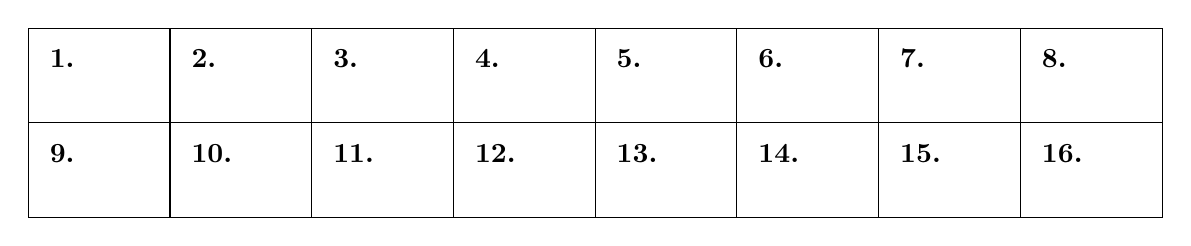
\begin{tikzpicture}[scale=1]
  % ---- 参数设置 ----
  \def\boxw{1.8} % 每个格子的宽度
  \def\boxh{1.2} % 每个格子的高度
  \def\gap{0} % 格子间距

  \def\offset{0.15} % 序号离边距离

  % ---- 16格答题栏：2行 × 8列
  \foreach \num in {1,...,16} {
    \pgfmathtruncatemacro{\row}{ifthenelse(\num<=8,0,1)}
    \pgfmathtruncatemacro{\col}{mod(\num-1,8)+1}
    \pgfmathsetmacro{\x}{(\boxw+\gap)*\col}
    \pgfmathsetmacro{\y}{-\row*(\boxh+\gap)}
    \draw (\x,\y) rectangle (\x+\boxw,\y+\boxh);
    \node[anchor=north west] at (\x+\offset,\y+\boxh-\offset) {\textbf{\num.}};
  }
\end{tikzpicture}
}

\end{flushleft}

% --- A部分：选择题 (开始) ---
\textbf{选择题：16题全做 \(40\%\)}

\begin{question}
    在平面直角坐标系中，将坐标原点平移至点 $O'(1, 2)$。若点 $P$ 在原坐标系下的坐标为 $(3, -2)$，则点 $P$ 在新坐标系下的坐标为： \paren[A]
    \begin{choices}
        \item $(2, -4)$ \item $(4, 0)$ \item $(2, 0)$ \item $(4, -4)$
    \end{choices}
\end{question}

\begin{solution}
    \textbf{解析：} \\
    设点 $P$ 的原坐标为 $(x, y) = (3, -2)$，新原点坐标为 $(h, k) = (1, 2)$。 \\
    根据平移坐标变换公式，新坐标 $(x', y')$ 满足 $x' = x - h$，$y' = y - k$。 \\
    代入数据得：$x' = 3 - 1 = 2$，$y' = -2 - 2 = -4$。 \\
    因此，点 $P$ 的新坐标为 $(2, -4)$。 \\
    故选 A。
\end{solution}

\begin{question}
    通过坐标轴平移，使原点移至点 $O'(h, k)$，若在此坐标变换下，曲线方程 $x^2 + y^2 - 4x + 6y + 9 = 0$ 在新坐标系中化简为 $x'^2 + y'^2 = 4$，则新原点坐标 $(h, k)$ 为： \paren[B]
    \begin{choices}
        \item $(-2, 3)$ \item $(2, -3)$ \item $(2, 3)$ \item $(-2, -3)$
    \end{choices}
\end{question}

\begin{solution}
    \textbf{解析：} \\
    将原曲线方程 $x^2 + y^2 - 4x + 6y + 9 = 0$ 进行配方，得： \\
    $(x^2 - 4x + 4) + (y^2 + 6y + 9) - 4 - 9 + 9 = 0$ \\
    即 $(x - 2)^2 + (y + 3)^2 = 4$。 \\
    要使其在新坐标系中的方程形式为 $x'^2 + y'^2 = 4$，则需令 $x' = x - 2$，$y' = y + 3$。 \\
    由平移公式 $x' = x - h$，$y' = y - k$ 对比可知，$h = 2$，$k = -3$。 \\
    因此，新原点坐标即平移向量 $(h, k)$ 为 $(2, -3)$。 \\
    故选 B。
\end{solution}

\begin{question}
    将直角坐标系绕原点逆时针旋转 $\frac{\pi}{4}$ 后，原坐标系下的曲线方程 $xy = 2$ 在新坐标系下的方程（选项中使用 $x, y$ 替代 $x', y'$ 表示新坐标）为： \paren[C]
    \begin{choices}
        \item $x^2 - y^2 = 2$ \item $x^2 + y^2 = 4$ \item $x^2 - y^2 = 4$ \item $y^2 - x^2 = 4$
    \end{choices}
\end{question}

\begin{solution}
    \textbf{解析：} \\
    设点在新旧坐标系下的坐标分别为 $(x, y)$ 和 $(x', y')$，旋转角 $\theta = \frac{\pi}{4}$。 \\
    根据坐标轴旋转公式，原坐标与新坐标的关系为： \\
    $x = x' \cos\frac{\pi}{4} - y' \sin\frac{\pi}{4} = \frac{\sqrt{2}}{2}(x' - y')$ \\
    $y = x' \sin\frac{\pi}{4} + y' \cos\frac{\pi}{4} = \frac{\sqrt{2}}{2}(x' + y')$ \\
    将上述式子代入原曲线方程 $xy = 2$ 中，得： \\
    $\frac{\sqrt{2}}{2}(x' - y') \cdot \frac{\sqrt{2}}{2}(x' + y') = 2$ \\
    即 $\frac{1}{2}(x'^2 - y'^2) = 2$，化简得 $x'^2 - y'^2 = 4$。 \\
    用 $x, y$ 替代 $x', y'$ 表示新坐标系下的方程，即为 $x^2 - y^2 = 4$。 \\
    故选 C。
\end{solution}

\begin{question}
    将坐标轴绕原点逆时针旋转 $\frac{\pi}{6}$ 后，得到新坐标系。若点 $P$ 在新坐标系下的坐标为 $(\sqrt{3}, 1)$，则点 $P$ 在原坐标系下的坐标为： \paren[B]
    \begin{choices}
        \item $(2, 0)$ \item $(1, \sqrt{3})$ \item $(\frac{3}{2}, \frac{\sqrt{3}}{2})$ \item $(\sqrt{3}, 1)$
    \end{choices}
\end{question}

\begin{solution}
    \textbf{解析：} \\
    已知旋转角 $\theta = \frac{\pi}{6}$，新坐标 $(x', y') = (\sqrt{3}, 1)$。 \\
    根据坐标轴旋转公式，原坐标 $(x, y)$ 的计算如下： \\
    $x = x' \cos\theta - y' \sin\theta = \sqrt{3} \cdot \cos\frac{\pi}{6} - 1 \cdot \sin\frac{\pi}{6} = \sqrt{3} \cdot \frac{\sqrt{3}}{2} - \frac{1}{2} = 1$ \\
    $y = x' \sin\theta + y' \cos\theta = \sqrt{3} \cdot \sin\frac{\pi}{6} + 1 \cdot \cos\frac{\pi}{6} = \sqrt{3} \cdot \frac{1}{2} + \frac{\sqrt{3}}{2} = \sqrt{3}$ \\
    因此，点 $P$ 在原坐标系下的坐标为 $(1, \sqrt{3})$。 \\
    故选 B。
\end{solution}

\begin{question}
    在极坐标系中，已知两点 $A(2, \frac{\pi}{6})$ 和 $B(4, \frac{\pi}{2})$，极点为 $O$。则 $\triangle AOB$ 的面积为： \paren[A]
    \begin{choices}
        \item $2\sqrt{3}$ \item $4$ \item $4\sqrt{3}$ \item $2$
    \end{choices}
\end{question}

\begin{solution}
    \textbf{解析：} \\
    在极坐标系中，设两点极坐标分别为 $(\rho_1, \theta_1)$ 和 $(\rho_2, \theta_2)$，则它们与极点构成的三角形面积公式为 $S = \frac{1}{2} \rho_1 \rho_2 \sin|\theta_1 - \theta_2|$。 \\
    代入已知数据：$\rho_1 = 2$，$ \theta_1 = \frac{\pi}{6}$；$\rho_2 = 4$，$ \theta_2 = \frac{\pi}{2}$。 \\
    两点极角之差为 $\Delta\theta = \frac{\pi}{2} - \frac{\pi}{6} = \frac{\pi}{3}$。 \\
    $\triangle AOB$ 的面积 $S = \frac{1}{2} \times 2 \times 4 \times \sin\frac{\pi}{3} = 4 \times \frac{\sqrt{3}}{2} = 2\sqrt{3}$。 \\
    故选 A。
\end{solution}

\begin{question}
    将极坐标方程 $\rho = 4\cos\theta$ 化为直角坐标方程，其结果是： \paren[A]
    \begin{choices}
        \item $x^2 + y^2 - 4x = 0$ \item $x^2 + y^2 + 4x = 0$ \item $x^2 + y^2 - 4y = 0$ \item $x^2 + y^2 + 4y = 0$
    \end{choices}
\end{question}

\begin{solution}
    \textbf{解析：} \\
    由极坐标与直角坐标的转换关系 $\rho^2 = x^2 + y^2$ 以及 $x = \rho\cos\theta$，$y = \rho\sin\theta$ 可知： \\
    将原极坐标方程 $\rho = 4\cos\theta$ 两边同时乘以 $\rho$，得到 $\rho^2 = 4\rho\cos\theta$。 \\
    将转换公式代入上式，可得 $x^2 + y^2 = 4x$。 \\
    移项整理后得到直角坐标方程为 $x^2 + y^2 - 4x = 0$。 \\
    故选 A。
\end{solution}

\begin{question}
    在极坐标系中，圆的方程为 $\rho = -6\sin\theta$，则该圆的半径为： \paren[B]
    \begin{choices}
        \item $6$ \item $3$ \item $9$ \item $-3$
    \end{choices}
\end{question}

\begin{solution}
    \textbf{解析：} \\
    将极坐标方程转化为直角坐标方程进行求解。 \\
    将 $\rho = -6\sin\theta$ 两边同乘 $\rho$，得 $\rho^2 = -6\rho\sin\theta$。 \\
    利用公式 $\rho^2 = x^2 + y^2$ 和 $y = \rho\sin\theta$，代入得 $x^2 + y^2 = -6y$。 \\
    移项并配方，得 $x^2 + (y^2 + 6y + 9) = 9$，即 $x^2 + (y + 3)^2 = 3^2$。 \\
    由此可知，该方程表示一个圆心在 $(0, -3)$，半径 $r = 3$ 的圆。 \\
    故选 B。
\end{solution}

\newpage
\vfill % 与上方内容保持距离

\noindent
\begin{tabular*}{\textwidth}{@{\extracolsep{\fill}} >{\centering\arraybackslash}p{0.22\textwidth} >{\centering\arraybackslash}p{0.22\textwidth} >{\centering\arraybackslash}p{0.22\textwidth} >{\centering\arraybackslash}p{0.22\textwidth}}
    出题： & 审题： & 审题： & 审核： \\[4em]
    \rule{6em}{0.5pt} & \rule{6em}{0.5pt} & \rule{6em}{0.5pt} & \rule{6em}{0.5pt} \\
    （蔡杰庆师） & （王萌师） & （张惠雯师） & （雷泳健师）
\end{tabular*}


\end{document}